\documentclass{standalone}

\usepackage[latin1]{inputenc}
\usepackage{tikz}

\usetikzlibrary{calc}

% GNUPLOT required
\begin{document}
\pagestyle{empty}



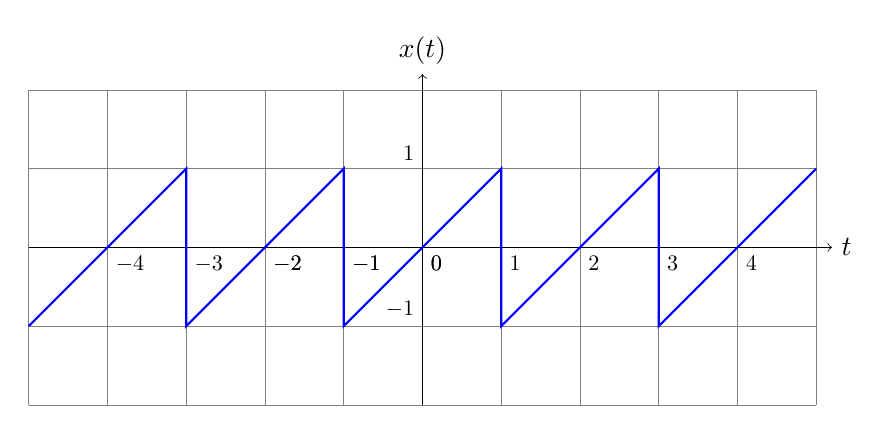
\begin{tikzpicture}[line width=0.3mm]
    \draw[very thin,color=gray] (-5,-2) grid (5,2);
    \draw[->, line width=0.1mm] (-5,0) -- (5.2,0) node[right] {$t$};
    \draw[->, line width=0.1mm] (0,-2) -- (0,2.2) node[above] {$x(t)$};

	% x(t)
	\draw[thick, color=blue] (-5,-1)--(-3,1)--(-3,-1)--(-1,1)--(-1,-1)--(1,1)--(1,-1)--(3,1)--(3,-1)--(5,1);

	\foreach \x in {-4,-3,...,0,...,3,4} {%
    \draw ($(\x,0) + (0,0)$) -- ($(\x,0) + (0,0)$)
        node [below right,scale=0.8] {$\x$};
	}
	\foreach \y in {-1,1} {%
    \draw ($(0,\y) + (0,0)$) -- ($(0,\y) + (0,0)$)
        node [above left,scale=0.8] {$\y$};
	}

\end{tikzpicture}


\end{document}
